% !TEX root = ./problem.en.tex
\gdef\thisproblemauthor{}
\gdef\thisproblemdeveloper{}
\gdef\thisproblemorigin{}
\begin{problem}{模數 Candy} %Note!
{standard input}{standard output}
{2 seconds}{512 MB}{}

Jill 最喜歡糖果了!\newline
為此她想開一間自己的糖果工廠來滿足無止盡的糖果欲!\\
\newline
這間工廠除了生產糖果以外還要兼顧美感和娛樂性,其中包裝糖果是個很重要的工作。\\
包裝的工作由一個巨大的包裝器負責,這個包裝器由 $N$ 道佇列組成,由左至右編號成 $0 \sim N-1$。每當包裝器收到一批剛產出的糖果,就會將這批糖果塞進其中一個佇列。每次包裝時,機器會選擇一個包裝大小 $v$ ,接著檢查編號 $L$ 至 編號 $R$ 的佇列 $(L\leq R)$,若發現任一佇列中的糖果數量 $ \geq v $ ,則讓該佇列落出 $v$ 個糖果裝入一個包裝,接著重複檢查數量、包裝直到範圍內的佇列都不足 $v$ 個糖果。\\
\centerline{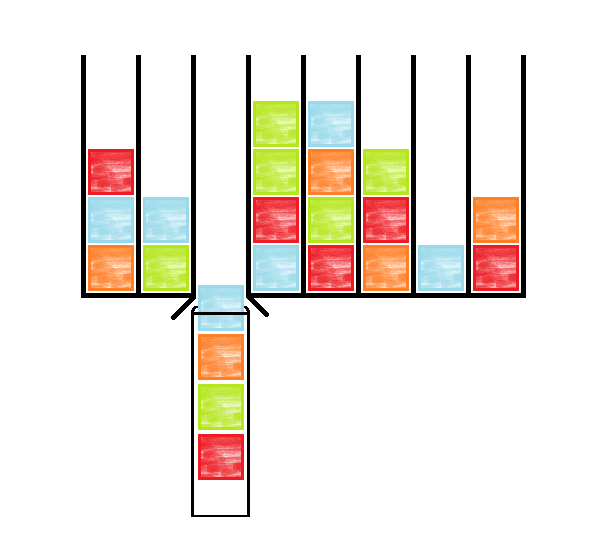
\includegraphics[height=22em]{./pics/E-1.png}}
\newline
為了確認生產過程的視覺效果,Jill 需要模擬生產行為,其中視覺效果的關鍵就在於佇列中的糖果堆放數量。Jill 將會給你 $M$ 個模擬事件、或詢問最大的堆放數量,詳細請參考 Input/Output 說明。\\
\newline
\InputFile

一個正整數 $N$ 表示佇列數量 \\
第二行有 $N$ 個非負整數 $a_0,a_1,...a_{n-1}$,表示各個佇列一開始堆放的糖果數量\\
下一行一個正整數 $M$ 表示接下來有 $M$ 個事件或來自 Jill 的詢問 \\
接下來 $M$ 行每行輸入一個事件或詢問 \\
每行第一個正整數 $K$ 表示發生了什麼樣的事件 \\
接著根據 $K$ 的數值有不同輸入,說明如下:
\begin{itemize}
\item $K=1$ $\Rightarrow$ [ 加入糖果\ ] \\
接著會輸入兩個正整數 $x$, $i$ \\
表示將 $x$ 個糖果放進編號 $i$ 的佇列\\
※每個佇列的容量都超大,不需要考慮滿出來的問題
\item $K=2$ $\Rightarrow$ [ 進行包裝\ ] \\
接著輸入三個整數 $L$,$R$,$v$ \\
 表示對編號 $L$ 到 編號 $R$ 的佇列要分別進行包裝大小為 $v$ 的包裝
\item $K=3$ $\Rightarrow$ [ Jill 的詢問\ ] \\
表示 Jill 想知道當前堆積最多糖果的佇列中有幾個糖果\\
這行沒有 $K$ 以外的輸入
\end{itemize}

\begin{iofmt}
\begin{itemize}
	\item $1 \leq N \leq 2\times 10^5$ %Note!
    \item $1 \leq M \leq 10^5$
    \item $1 \leq a_i \leq 10^8$
    \item $1 \leq x \leq 10^4$
	\item $0 \leq L \leq R < N$
	\item $1 \leq v \leq 10^6$
    \item $0 \leq i < N$
	\item 有 3 分的測試資料 $N \leq 100$
	\item 有 22 分的測試資料 $K \in \{1,3\}$
\end{itemize}
\end{iofmt}

\OutputFile

對於 Jill 的每個詢問,輸出一行\\
每行一個正整數,表示最多糖果的佇列有幾個糖果

\Examples

\begin{example}
 \exmpfile{./sample/PE-01.in.txt}{./sample/PE-01.out.txt}%
% \exmpfile{./sample/PC-02.in.txt}{./sample/PC-02.out.txt}%
\end{example}

\end{problem}
